\documentclass[
	a4paper, % Paper size, use either a4paper or letterpaper
	10pt, % Default font size, can also use 11pt or 12pt, although this is not recommended
	unnumberedsections, % Comment to enable section numbering
	twoside, % Two side traditional mode where headers and footers change between odd and even pages, comment this option to make them fixed
]{LTJournalArticle}

\addbibresource{sample.bib} % BibLaTeX bibliography file

% A shortened article title to appear in the running head, leave this command empty for no running head

% \footertext{\textit{Journal of Biological Sampling} (2024) 12:533-684} % Text to appear in the footer, leave this command empty for no footer text

\setcounter{page}{1} % The page number of the first page, set this to a higher number if the article is to be part of an issue or larger work

%----------------------------------------------------------------------------------------
%	TITLE SECTION
%----------------------------------------------------------------------------------------

\title{Design Exercise 2\\ Engineering Notebook} % Article title, use manual lines breaks (\\) to beautify the layout

% Authors are listed in a comma-separated list with superscript numbers indicating affiliations
% \thanks{} is used for any text that should be placed in a footnote on the first page, such as the corresponding author's email, journal acceptance dates, a copyright/license notice, keywords, etc
\author{%
	Adarsh Hiremath and Andrew Palacci
}


%----------------------------------------------------------------------------------------

\begin{document}

\maketitle % Output the title section

%----------------------------------------------------------------------------------------
%	ARTICLE CONTENTS
%----------------------------------------------------------------------------------------

\section{I. Introduction}
In our design exercise, we implemented a model of a small, asynchronous distributed system. In this system, each of the three simulated machines run at different clock rates assigned randomly at initialization. Each machine listens on a socket for incoming messages from other machines and updates its corresponding logical clock and message queue. In this engineering notebook, we intend to describe our design decisions when building this model, and the results from the following experiments:
\begin{itemize}
    \item Five iterations of the scale model for exactly one minute. 
    \item A single run of the scale model for two minutes.
    \item Three trials where we modify the probabilities that machines send messages to other machines. 
\end{itemize}

The source code for our chat application can be found \href{https://github.com/andrewp2303/logical_clocks}{here}.

\section{II. Model Distributed System Design}

Building our scale model for the simulated machines required implementing a protocol for the three machines to communicate. Otherwise, it would be impossible to receive logical clock information, send messages, or update the message queue. Thus, the first question we sought to answer in the design process was what protocol we wanted to implement for our scale model. 

Initially, we were inclined to implement our communication protocol using a simple peer-to-peer (P2P) networking library such as \href{https://pypi.org/project/pyp2p/}{Python's P2P}. The idea of P2P networking was appealing since there would be no single point of failure;  each machine could act as both a client and server, allowing for a more dynamic and flexible system. Additionally, with P2P, we thought that we could cut the number of connections in half because every connection would be bidirectional. 

However, we decided to use web sockets instead for a couple of reasons: 
\begin{itemize}
    \item By using web sockets, we could partially reuse implementations from the first design project instead of learning P2P networking for the first time for this project. 
    \item The problem specification recommended that each machine in the simulation send and receive information using web sockets. 
    \item Completely decentralizing communication is not realistic, especially at scale. It is far easier to accommodate more machines in a distributed system without dramatically revamping the code base when machines can ping a server with just one endpoint. Thus, we wanted to make something that emulated the pairwise nature of P2P networks, while using sockets to ensure extensibility to a centralized model when issues of scale arose.
\end{itemize}

For these reasons, instead of using a P2P system we decided to have each machine create 2 socket connections --- one to each of the other machines. Additionally, each machine has one socket "server," which is used exclusively to listen for incoming messages using $consumer$ threads. Furthermore, the other two sockets are used exclusively to send outgoing messages to the other machines in the model. Since we implemented the previous design project in Python, we did the same for this design project as well. 

Finally, a pivotal design decision we made was deciding to implement our exercise with pairwise socket connections, instead of using a centralized server. Here were some of the considerations for doing so: 
\begin{itemize}
    \item We noted that using a centralized server would greatly reduce our initialization costs --- we would only need to form $n$ socket connections (in this case 3), as opposed to $2{n \choose 2}$ (in this case 6) if we wanted to connect every machine to every other machine. Note that the second option is an order of magnitude more expensive, but that this is still a one-time cost. 
    \item We then noted that the runtime costs of using a server would be twice as high, because the server would need to both receive and distribute messages. This would be reasonable if we had a very powerful server, but in this exercise we assumed machines that were performing similarly. Thus, as we see in the experiments later on, if we labeled one of the machines as the server it could result in that machine being unable to manage every machine's request --- this would constitute a bottleneck and a single point of failure, instead of independent failures of each machine and distributed transactions. This was the deciding factor for our decision-making, since the risk of extreme slowdowns or even total failure far outweighed the benefit of a lowered initialization cost.
\end{itemize}

\section{III. Five Scale Model Iterations}

We ran five simulations of our model distributed system, each for approximately a minute. During each simulation, we logged the message queue size and logical clock time for each machine after every completed tick of the machine. 
    
Initially, we logged the message queue size and logical clock time using Python's time module. However, unreliability in the time module and differences across machines prompted us to utilize the tick times from the simulations themselves. We initialized a variable, \texttt{currTime}, to 0 at the start of every thread. Then, at every operation, we incremented \texttt{currTime} until it hit the randomly generated \texttt{tickSize} for each machine. Then, we set \texttt{currTime} to 0 once again, repeating the process. Since each machine runs at a clock rate of 0 to 6 ticks per second, we were effectively able to simulate one "real" second on each simulated machine to log any necessary values for producing our graphs. 

On the next page, we illustrate our 5 trials of this experiment from the exercise specification, including the clock speed of each process for each experiment.  

\newpage
$$ $$
\newpage
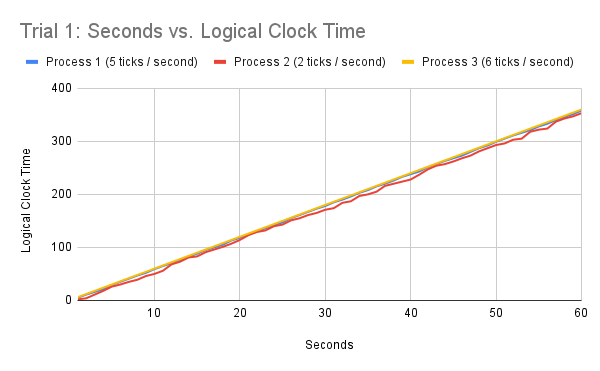
\includegraphics[width=7.8cm]{assets/t1_clock.png}
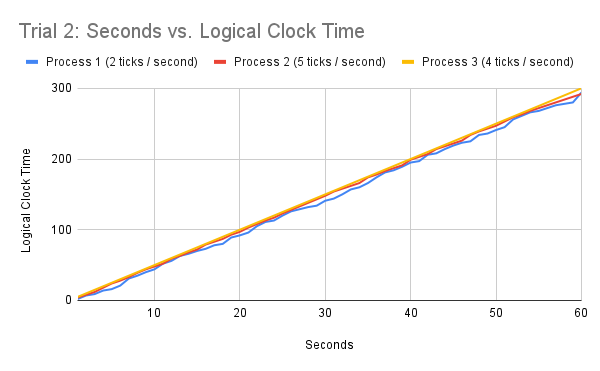
\includegraphics[width=7.8cm]{assets/t2_clock.png}
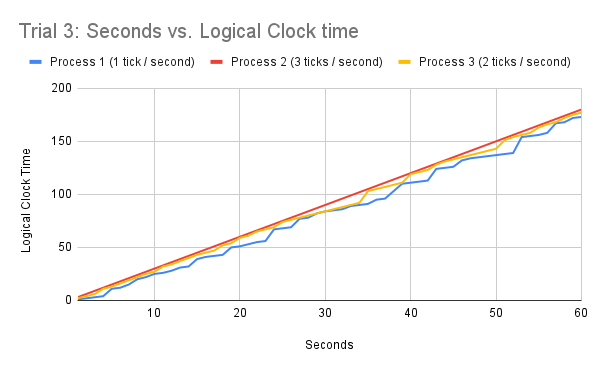
\includegraphics[width=7.8cm]{assets/t3_clock.png}
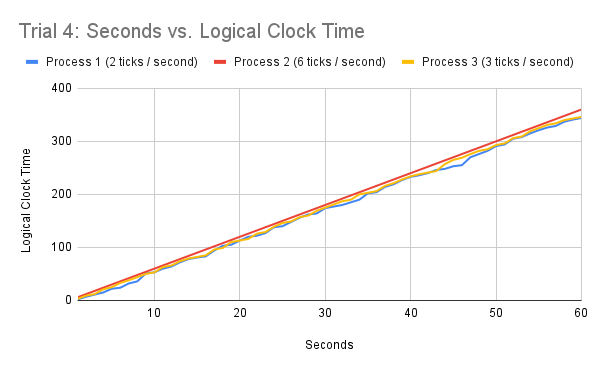
\includegraphics[width=7.8cm]{assets/t4_clock.png}
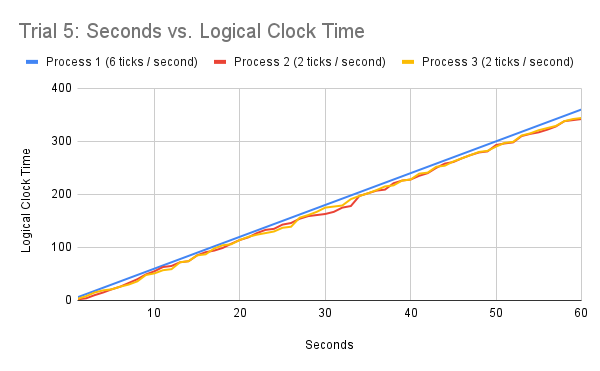
\includegraphics[width=7.8cm]{assets/t5_clock.png}
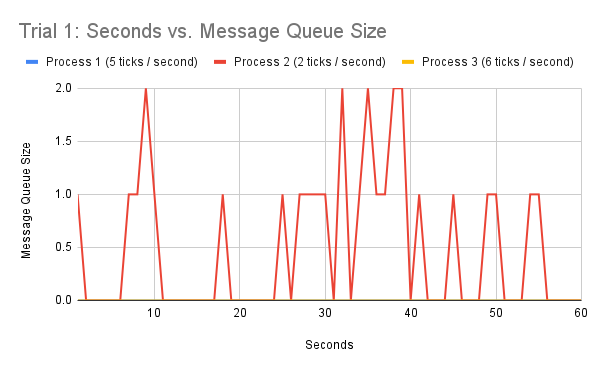
\includegraphics[width=7.8cm]{assets/t1_size.png}
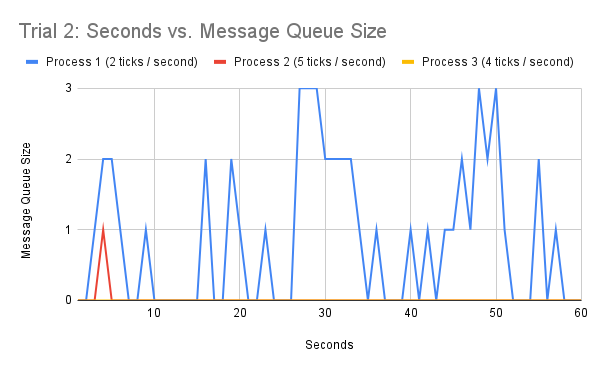
\includegraphics[width=7.8cm]{assets/t2_size.png}
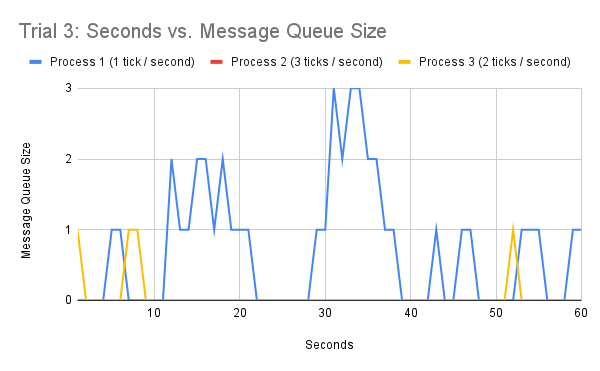
\includegraphics[width=7.8cm]{assets/t3_size.png}
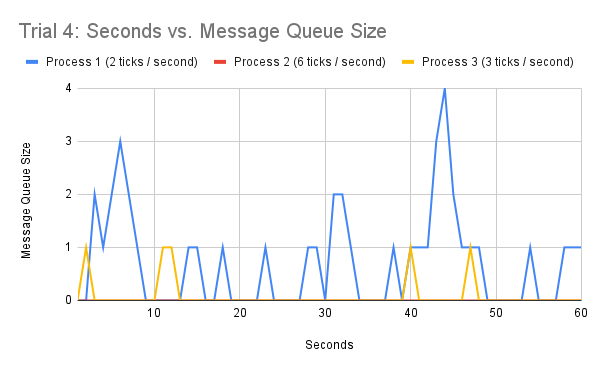
\includegraphics[width=7.8cm]{assets/t4_size.png}
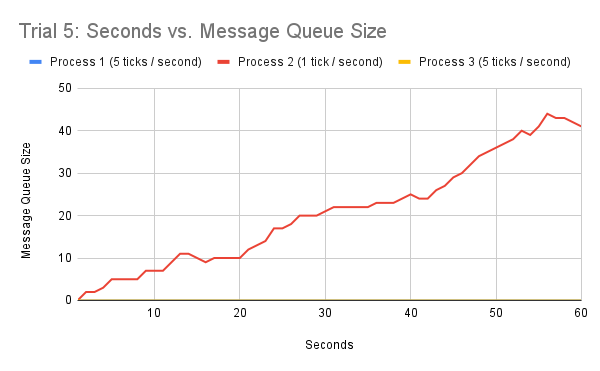
\includegraphics[width=7.8cm]{assets/t5_size.png}

\vspace{1mm}

After experimenting with our scale models and analyzing the above graphs, we noticed the following important trends: 
\begin{itemize}
    \item Processes runnning at fewer ticks per second had much larger jumps in logical clock time. This is best illustrated on the graph for trial 3 where process 1 ran at 1 tick / second, process 2 ran at 3 ticks / second, and process 3 ran at 2 ticks / second. The line for process 1 is the most jagged, demonstrating larger deviations  from the top line. The line for process 3 is the second most jagged, with the line for process 2 setting an effective linear upper bound for logical clock time. The jaggedness/variance in these lines exponentially reduces, demonstrating that faster tick speeds also reduce variations in logical clock time. This makes sense, because the fastest machine should usually lead the rest of the machines, explaining why the fastest machine appears as linear.
    \item Processes running at fewer ticks per second also struggled to manage the message queue. This is illustrated well in the message queue graph for trial 1, where every process except the one running at 2 ticks / second had a queue length of 0 for the entirety of the simulation. This is logical because systems operating at a slower clock speed struggle to process inbound messages of peers running at comparatively higher clock speeds, thus sending more messages. Notice that in this case, the queue size still oscillates from 0 to some constant --- this is acceptable behavior, since the logical clocks stay mostly in sync relative to real time. This indicates that message queue buildup is due not only to the rate at which other machines run, but also the probability that they will send a given machine a message on each run. 
    \item The behavior for the logical clock and message queue size radically changes when two processes are running at a much higher speed than the other process. In Trial 5, for example, two processes are running at 5 ticks / second while the remaining process is running at 1 tick / second. For the slowest process, the message queue continues to fill up and accumulate because the process can deal with only one message per second, but it's being sent an expected 2 messages per second. Thus, even though the logical clock is still technically working and Process 2 is respecting the causality of messages that were sent to it, we know from a gods-eye view that even after a minute there is a very significant discrepancy between logical clock times at the current real time. This shows that discrepancies in logical clock vs. real time correspond directly to buildup in a message queue.
\end{itemize}

\section{IV. Longer Scale Model Iterations}

In order to test our model further, we ran several extended tests, including another iteration for 2 minutes instead of 1 minute to verify the behavior of the logical clock and message queue size. We generated the following graphs for this longer iteration: 

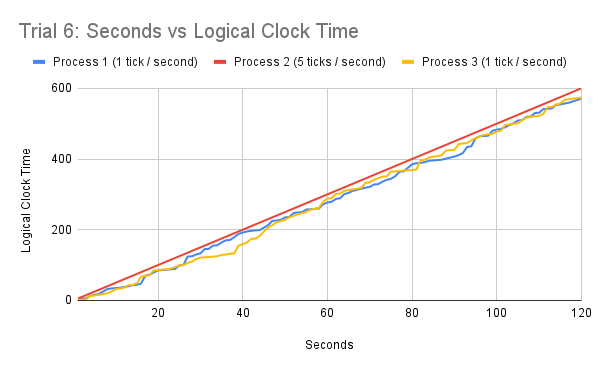
\includegraphics[width=7.8cm]{assets/t6_clock.png}
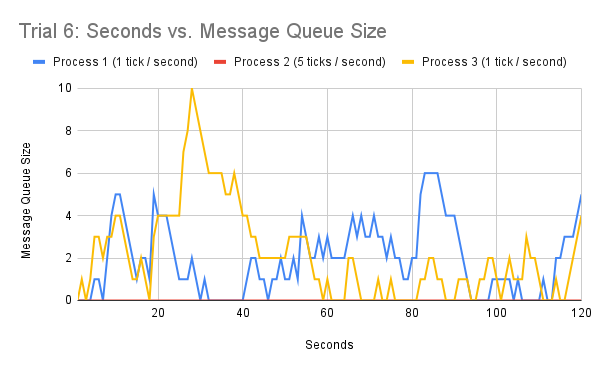
\includegraphics[width=7.8cm]{assets/t6_size.png}

In the above graphs, we observe the inverse of the case in trial 5: there are two extremely slow processes and one extremely fast process. The graph behavior is consistent with our expected behavior since the jaggedness of the logical clock graph varies identically to the 1 minute case (a smaller clock cycle results in a higher variance of jumps in logical clock times). Additionally, we observe the expected behavior in the message queue graph with the two processes running at 1 tick / second spiking. The message queue size for the 2 minute case also appears to a linear factor away from the message queue in the 1 minute case for a comparable set of process ticks / second.

\section{V. Modified Probabilities}

In our final set of experiments, we modified the probabilities of our simulated machines sending messages. In trial 7 and 8, we used a (1, 5) range instead of a (1,10) range when determining whether to send a message, resulting in a higher hit rate. In trial 9, we used a (1,15) range when determinining whether to send a message, resulting in a lower hit rate. 

We generated the following graphs: 

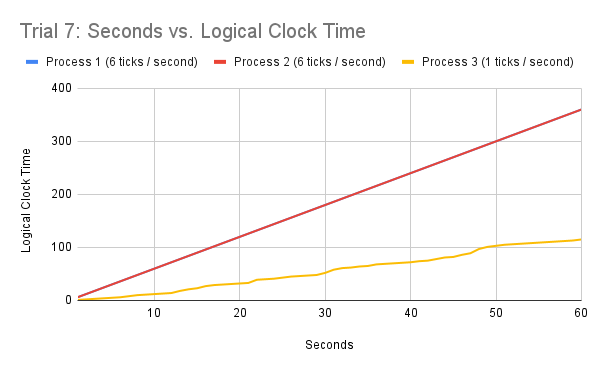
\includegraphics[width=7.8cm]{assets/t7_clock.png}
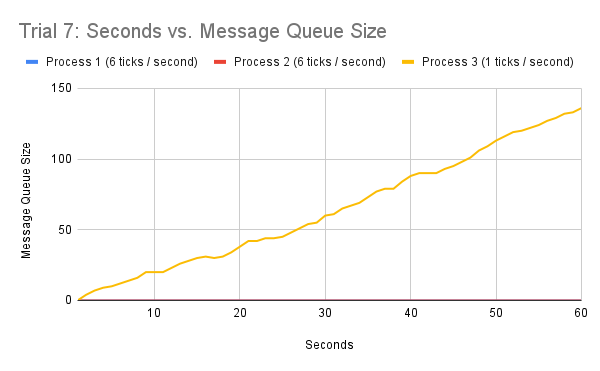
\includegraphics[width=7.8cm]{assets/t7_size.png}
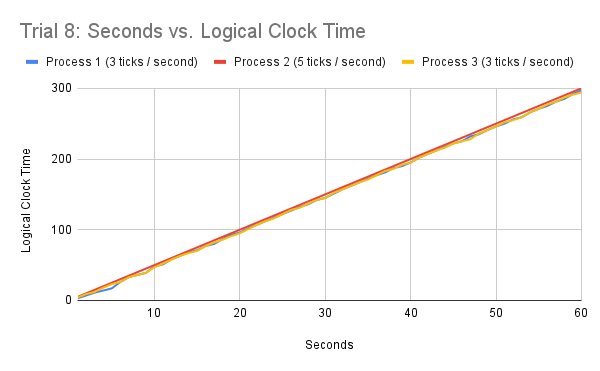
\includegraphics[width=7.8cm]{assets/t8_clock.png}
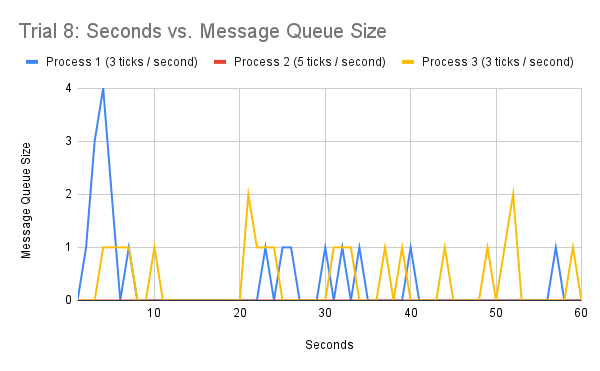
\includegraphics[width=7.8cm]{assets/t8_size.png}
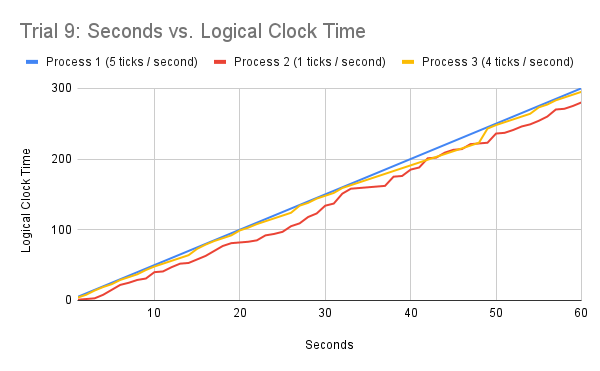
\includegraphics[width=7.8cm]{assets/t9_clock.png}
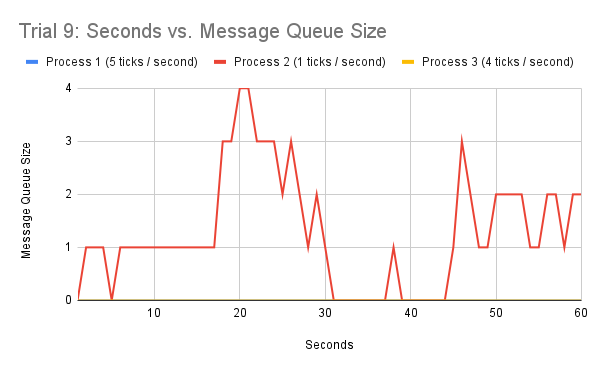
\includegraphics[width=7.8cm]{assets/t9_size.png}

From these graphs, we noticed the following important trends: 
\begin{itemize}
    \item When there is a higher hit rate, the message queue loads up at a faster rate than observed in trials 1-5. An example that illustrates this is trial 7. Here, there are two extremely fast processes with clock rates of 6 ticks / second and one extremely slow process with a clock rate of 1 tick / second. The lag from the slow process is incredibly large, with the process reaching less than half the logical clock time as the 6 ticks / second processes over the same time interval. Like in trial 5, causality is preserved, but the slow process is spammed to the point where it is stuck handling old message requests.
    \item The message queue varies more when the differences in the clock rate are more extreme. However, the message queue variations aren't as pronounced when the differences in the clock rate aren't extreme. 
    \item The logical clock of the slowest process is able to keep up with substantially faster processes when the hit rate is lower. This is shown in trial 9 where the two fast processes run at 5 ticks / second and 4 ticks / second, while the slow process runs at 1 tick / second. Despite this variance in clock speeds, the slow process and the faster processes have the same logical clock time after the 1 minute period. In trials 5 and 7, however, the message queue was overloaded and the logical clock of the slowest process was not able to keep up with the faster processes over the same time interval. 
    
\end{itemize}


\section{VI. Unit Testing}
Finally, we made sure to test our application for robustness against non-Byzantine errors and for correct behavior. First, we realized that our program contained in \texttt{clocks.py} does not have any input-output methods, and instead runs worker methods in several processes and threads that don't return, which either modify data structures (such as our message queue) or print to files (such as $log\{PORT\}.txt$). Thus, we decided the most logical way to test would be using assertions within each method, mainly focusing on tests that our messages were sent and received in a valid format, and that inputs to methods were well-formed. Thus we first checked the validity of configurations before passing them into our "machines" (e.g. processes running the machine method):
\begin{python}
def assertConfig(config):
	'''Check that an input config is valid.'''

	# Validate host address using a regex.
	# https://www.geeksforgeeks.org/python-
	# program-to-validate-an-ip-address/.
	ipRegex = "^((25[0-5]|2[0-4][0-9]|1[0-9]
			[0-9][1-9]?[0-9])\.){3}"
	ipRegex += "(25[0-5]|2[0-4][0-9]|1[0-9]
			[0-9]|[1-9]?[0-9])$"
	assert(type(config[0]) == str)
	assert(re.match(ipRegex, config[0]))

	# Check that port is in valid range, and 
	# that tick size is at least 1.
	assert(type(config[1]) == int)
	assert(config[1] >= 0 and 
		config[1] <= 65535)
	assert(type(config[2]) == int)
	assert(config[2] >= 1)
\end{python}

We also made sure to test the "payload" upon reception through a socket connection --- note that this payload is just a possible logical clock value, so we used the following two tests:
\begin{python}
	assert(dataVal.isnumeric())
	assert(int(dataVal) >= 0)
\end{python}

We noted that since our logical clock is declared as an integer, this remains invariant, and thus we didn't need to test whether messages were well-formed, because they were just the logical clock value. However, in every area of the code where such claims were less obvious, we made sure to add assertions (all of which passed during runtime). 

Additionally, we used the try-except structure when connecting to sockets, and returned an error message, adding robustness to our program. We also performed other validations, such as checking whether a message received in a consumer thread was empty before adding it to the message queue. 
\newpage Here is one example of the former below:
\begin{python}
try:
	s.connect((HOST,port))
	sockets.append(s)
	print("Client-side connection success 
			to port val:" + str(port) + "\n")

except socket.error as e:
	print("Error connecting producer: %s" % e)
\end{python}



\end{document}
